\section{Standard Bitcoin Network}\label{sec:general-poc}

This section provides an analysis of a Bitcoin network configured with standard
nodes and miners that create blocks, generate transactions, and propagate them
throughout the network. The analysis will also be used to perform validation of
the model proposed in this work.

\subsection{The Model}\label{subsec:general-model}

The model used for this analysis has the following characteristics:
\begin{itemize}
	\item 50 user nodes that create transactions at an average rate of 1
		transaction every 20 seconds;
	\item 10 miner nodes, each with varying hash rates, also generating
		transactions at an average rate of 1 transaction every 20
		seconds;
	\item 1 user node creating transactions at a slower rate of 1
		transaction every 5 minutes (300 seconds);
	\item 1 user node generating transactions at a faster rate of 1
		transaction per second.
\end{itemize}

In total, the network consists of 62 nodes, producing slightly over 4
transactions per second globally. The mean rate of transactions added to the
mempool before 2023 was approximately 4--5 transactions per second. Recently,
this rate has increased to around 6--7 transactions per second due to the
cryptocurrency's rise in popularity during the ongoing \emph{bull} market
period (2023--2024) \cite{blockchaincom-tps}. However, it is essential to note
that since 2017, Bitcoin has supported \emph{Segmented Witness} (SegWit)
transactions, which enhance throughput, whereas \iblock{} currently lacks
SegWit support, making such throughput levels impractical within this simulated
network \cites{bip141, bip144}. Before the SegWit adoption, the Bitcoin network
was restricted to a sustained rate of 7 transactions per second due to the
bitcoin protocol restricting block sizes to 1 MB \cite{btcwiki-scalability}. 


The 10 miners in this scenario have the following hash rate distributions (in
percentage): \(0.1\%\), \(0.4\%\), \(0.5\%\), \(1\%\), \(3\%\), \(5\%\),
\(10\%\), \(15\%\), \(25\%\) and \(40\%\). This configuration allows for a
diverse range of hash rates, facilitating the analysis of miners with both low
and high computational power.

The simulation duration is set to 3 days, with 30 runs performed using
different random seeds. This configuration is labeled as ``StandardBitcoin''
within the \texttt{simulations/pocs.ini} file.

\subsection{Result Analysis}\label{subsec:general-analysis}

Across the 30 simulations, the mean number of blocks mined was \(425.57\),
close to the expected \(6 \times 24 \times 3 = 432\) blocks (based on the
average of six blocks per hour that the bitcoin protocol tries to enforce)
\cite[Chapter~``Difficulty'']{learnmeabitcoin}. The minimum number of blocks
mined was \(381\), and the maximum was \(468\), indicating that \iblock{}
accurately models the Proof-of-Work (PoW) mining process within the network.

\figref{fig:general-blocks-mined} illustrates the number of blocks mined by
each miner. The red horizontal line represents the expected number of blocks
per miner, calculated by multiplying the expected total number of mined blocks
(\(432\)) by each miner’s respective hash rate percentage. Notably, all
\(95\%\) confidence intervals include the expected block count, confirming
simulation consistency with theoretical values.

\begin{figure}[tbhp]
	\centering
	\includegraphics[width=\textwidth,trim={2.95cm 1.85cm 3.3cm
			2.5cm},clip]{standard-blocks-mined}
	\caption{Number of blocks mined by each miner. Confidence intervals at
	\(95\%\) level, with 30 samples. Red lines represent expected
	theoretical values.}\label{fig:general-blocks-mined}
\end{figure}

Miners with higher hash rates mined more blocks and, consequently, received
greater rewards. \figref{subfig:general-rewards} shows the mining rewards (in
satoshis) per miner, while \figref{subfig:general-balance} displays the final
wallet balances (also in satoshis) for each miner. These bar charts resemble
the distribution seen in \figref{fig:general-blocks-mined}, as miners did not
earn additional funds from transactions sent by other nodes, given that all
nodes, including miners, act as both transaction senders and receivers,
effectively balancing out the amount of received bitcoins with those that they
send out.

\begin{figure}[tbhp]
	\centering
	\begin{subfigure}[b]{0.49\textwidth}
		\centering
		\includegraphics[width=\textwidth,trim={3.05cm 1.85cm 3.3cm
			2.5cm},clip]{standard-rewards}
		\caption{Mining rewards (in satoshis) per miner, including
		block subsidies and fees.}\label{subfig:general-rewards}
	\end{subfigure}
	\begin{subfigure}[b]{0.49\textwidth}
		\centering
		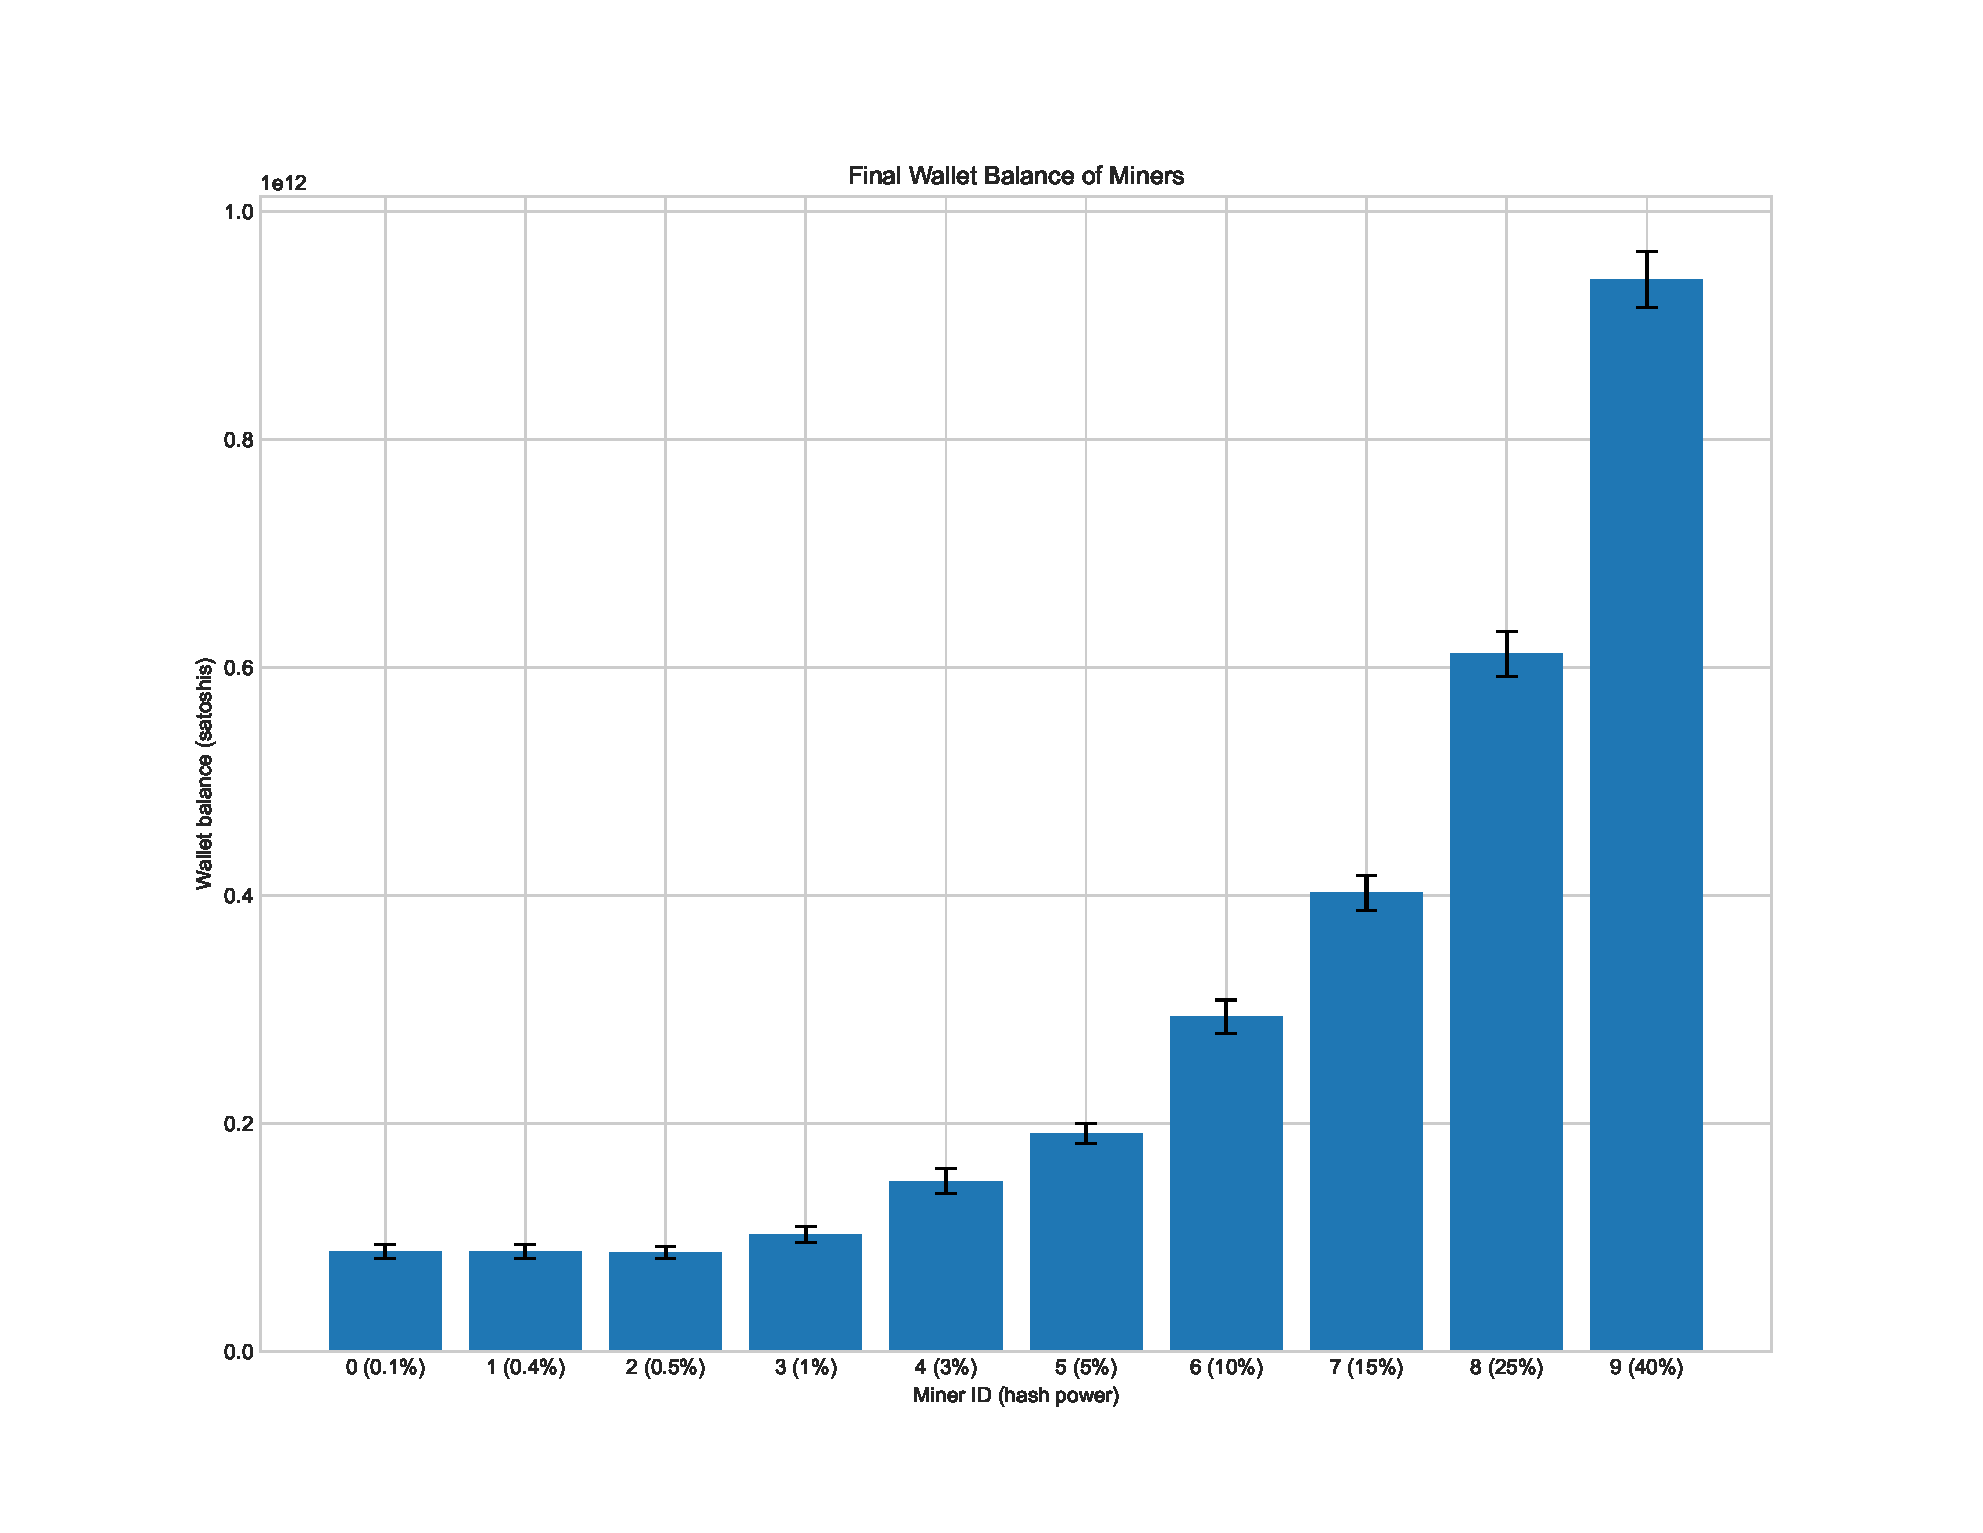
\includegraphics[width=\textwidth,trim={3.05cm 1.85cm 3.3cm
			2.5cm},clip]{standard-balance}
		\caption{Final wallet balance (in satoshis) for each
		miner.}\label{subfig:general-balance}
	\end{subfigure}
	\caption{Mining rewards and final wallet balances per miner, with
	\(95\%\) confidence intervals based on 30
	samples.}\label{fig:general-rewards-balance}
\end{figure}

\figref{subfig:general-transactions} shows the number of transactions generated
by each network node. The first 10 bars correspond to miners, the
11\textsuperscript{th} bar represents the node generating transactions every 5
minutes, the 12\textsuperscript{th} bar represents the node generating
transactions every second, and the remaining 50 bars represent standard nodes.
As expected, nodes generate similar numbers of transactions, except for the two
nodes with modified rates.

The 60 nodes producing transactions at the standard rate created an average of
\(12963.1\) transactions each, consistent with the theoretical \(3 \times 60
\times 24 \times 3 = 12960\) transactions over three days (three transactions
per minute). The node creating transactions every 5 minutes generated an
average of \(865.47\) transactions, matching the expected \(12 \times 24 \times
3 = 864\) transactions over three days. The node generating transactions every
second created an average of \(259054.63\) transactions, aligning with the
expected \(60 \times 60 \times 24 \times 3 = 259200\) (the total seconds over
three days). The sum of mean transactions across all nodes was \(1037706.13\),
equivalent to approximately \(4.0035\) transactions per second, validating the
transaction generation model in the simulation.


\figref{subfig:general-paid-fees} displays the total transaction fees paid by
each node. The node generating transactions every second paid significantly
higher fees due to its high transaction volume, while the node with the slower
transaction rate incurred lower fees. All other nodes paid similar fees,
reflecting their uniform transaction generation rates.

\begin{figure}[p]
	\centering
	\begin{subfigure}[b]{0.85\textwidth}
		\centering
		\includegraphics[width=\textwidth,trim={2.35cm 1.85cm 3.3cm
			2.5cm},clip]{standard-transactions}
		\caption{Transaction count per
		node.}\label{subfig:general-transactions}
	\end{subfigure}
	\par\bigskip\medskip
	\begin{subfigure}[b]{0.85\textwidth}
		\centering
		\includegraphics[width=\textwidth,trim={3.05cm 1.85cm 3.3cm
			2.5cm},clip]{standard-fees}
		\caption{Total transaction fees paid by each node (in
		satoshis).}\label{subfig:general-paid-fees}
	\end{subfigure}
	\caption{transaction counts and fees paid by each node, with \(95\%\)
	confidence intervals based on 30
	samples.}\label{fig:general-transactions-fees}
\end{figure}
